%格式設定%
\documentclass[a4paper,12pt]{article}
\usepackage[utf8]{inputenc}
\usepackage{xeCJK}
\usepackage{fontspec}
\usepackage{graphicx}
\usepackage{float}
\usepackage{hyperref}
\usepackage{mathtools}
\usepackage[margin=1cm]{geometry}
\setmainfont{Times New Roman}
\setCJKmainfont{kaiu.ttf}
\linespread{1.5}

\title{\LaTeX 學習筆記}
\author{方若堯}

\begin{document}
\maketitle
\section{學習動機}
以前使用Word、Google docs等文書處理軟體時常出現不好排版，諸如文字對齊或圖片容易跑掉等情況。
加上LaTeX數學公式的處理能力很強，之後若要寫報告、論文也用的到，故產生了用自主學習時間學習LaTeX的想法。

\section{LaTeX簡介}
一種建立在TeX之上的排版工具，由美國電腦科學家Leslie Lamport在1980年代初期開發。
他設計LaTeX的初衷就是要讓完全不懂程式或排版的使用者也能快速產出專業水準的文件。
採用純文字編輯加上特定命令標記的方式來撰寫文件。
因其強大的公式、圖表產生能力常被用在各種理工科的報告、論文等。

\section{開發環境}
因為平常就會用vscode寫程式之類的，所以選它當作開發環境。
總之先到官網下載Latex的發行版(我這裡使用MiTeX)，接著安裝到本地。然後下載Perl(我使用的是Strawberry Perl)，把它丟進環境變數裡。
接著vscode下載LaTeX Workshop，然後因為會使用中文編輯，排版引擎使用XeTeX，所以將xelatexmk移至recipe的最上行以將其作為預設。
\begin{figure}[H]
    \centering
    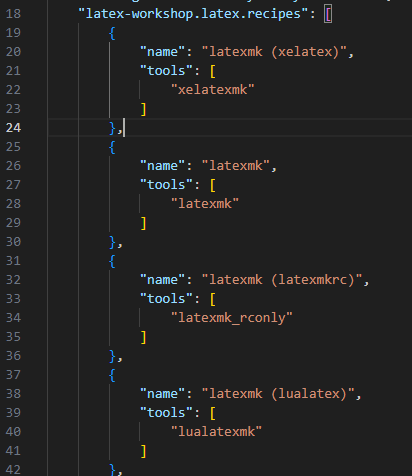
\includegraphics[width=0.3\textwidth]{F1.png}
\end{figure}
接著就是寫一個HelloWorld出來測試:
\begin{figure}[H]
    \centering
    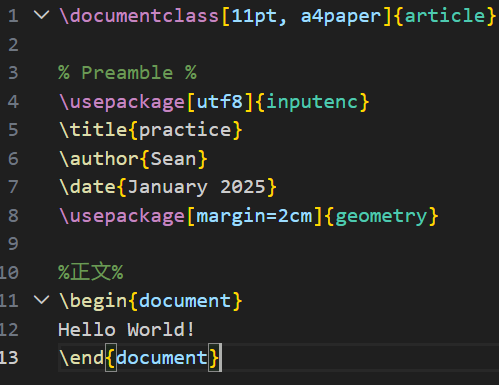
\includegraphics[width=0.5\textwidth]{HelloWorld.png}
\end{figure}

\section{基本指令及格式設定}
基本語法:使用\verb|指令由\開頭，[]中為選擇性參數，{}中的參數不能忽略。|另外註解是以\% 包裹。 \\
標示文件開頭及結尾:\verb|\begin{document} 中間是文章內文 \end{document}| \\
設定文件格式及用紙、字體大小等:\verb|\documentclass[a4paper(用紙), 11pt(字體大小)]{article(文件格式，還有book、letter等)}| \\
設定英文字體(中文字體後述):\verb|\setmainfont{Times New Roman}| \\
設定行距:\verb|\linespread{1.5(行距為預設之1.5倍)}| \\
基本分段:\verb|\chapter > \part > \section > \subsection| \\
換行:\verb|\| \\
空格符號:\verb|\ | \\
插入純文字:\verb|\verb| \\
\section{引入中文}
使用xeCJK套件，然後輸入\verb|\setCJKmainfont{字型代號}|
\section{表格及圖片}
表格我通常是用tabular做，範例如下: \\
\begin{verbatim}
    \begin{tabular}{c|cc}
    1 & 2 & 3 \\
    \hline
    item & item & item \\
    item & item & item \\
    \end{tabular}
\end{verbatim}
\qquad $\downarrow$ \\
\begin{tabular}{c|cc}
    1 & 2 & 3 \\
    \hline
    item & item & item \\
    item & item & item \\
\end{tabular} \\
\verb|{c| | \verb|cc}|中的c是代表將表格中的內容置中對齊，|是代表分隔線。表格中的物件以\&分隔，換行一樣由\verb|\\|表示。
\verb|\hline|表示橫的分隔線，因為它有內建換行所以不用在後面加\verb|\\|。 \\
圖片插入要以\verb|\begin{figure}|宣告，注意這裡要用的圖片需與.tex檔位於同一資料夾且須使用graphicx套件。指令如下: \\
\begin{verbatim}
\begin{figure}[H]
    \centering
    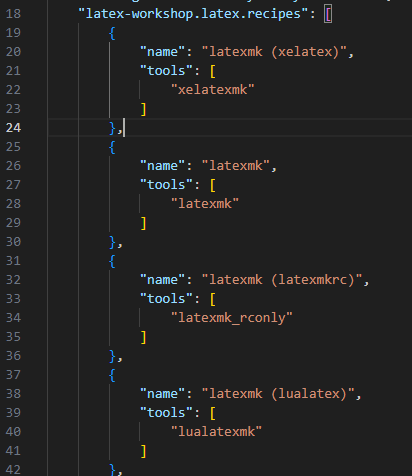
\includegraphics[width=0.3\textwidth]{F1.png}
\end{figure} \\
其中[H]表示使圖片不隨文字移動，\verb|\centering|表示將圖片置中，\verb|\includegraphics[width=0.3\textwidth]{圖檔名}|表示匯入圖片並將其以0.3的倍率顯示。
\end{verbatim}
\section{插入連結}
使用hyperref套件，指令為\verb|\url{連結}|，另外hyperref也可以做文件內的超連結。
\section{常用數學公式}
這裡使用mathtools套件 \\
公式指令的前後要以\verb|$$|包圍以使用mathjax渲染。
也可使用\verb|\begin{math}(行內公式|或\verb|begin{displaymath}(行間公式)| \\
1. 二元運算 \\
\\
\begin{tabular}{|c|c|c|c|c|c|c|c|c|}
    \hline
    預覽 & $+$ & $-$ & $\times$ & $\div$ & $\setminus$ & $\pm$ & $\mp$ & $\cdot$ \\
    \hline
    指令 & \verb|+| & \verb|-| & \verb|\times| & \verb|\div| & \verb|\setminus| & \verb|\pm| & \verb|\mp| & \verb|\cdot| \\
    \hline
\end{tabular} \\
2. 二元關係 \\
\\
\begin{tabular}{|c|c|c|c|c|c|c|c|}
    \hline
    預覽 & $>$ & $<$ & $=$ & $\le$ & $\ge$ & $\sim$ & $\approx$  \\
    \hline
    指令 & \verb|>| & \verb|<| & \verb|=| & \verb|\le| & \verb|\ge| & \verb|\sim| & \verb|\approx|  \\
    \hline
    預覽 & $\subset$ & $\supset$ & $\subseteq$ & $\supseteq$ & $\in$ & $\ni$ & $\propto$ \\
    \hline
    指令 & \verb|\subset| & \verb|\supset| & \verb|\subseteq| & \verb|\supseteq| & \verb|\in| & \verb|\ni|& \verb|\propto| \\
    \hline
\end{tabular} \\
另外，可以在指令前加上\verb|\not|產生其否定。 \\
3. 邏輯符號 \\
\\
\begin{tabular}{|c|c|c|c|c|c|c|c|c|}
    \hline
    預覽 & $\forall$ & $\exists$ & $\And$ & $\land$ & $\wedge$ & $\neg$ \\
    \hline
    指令 & \verb|\forall| & \verb|\exists| & \verb|\And| & \verb|\land| & \verb|\wedge| & \verb|\neg| \\
    \hline
\end{tabular} \\
4. 上標、下標 \\
\\
\begin{tabular}{|c|c|c|c|c|c|}
    \hline
    預覽 & $a^{m}_{n}$ & $\overline{m+n}$ & $\overbrace{m+\cdots+n}^{10}$ & $\overrightarrow{mn}$ \\
    \hline
    指令 & \verb|a^{m}_{n}| & \verb|\overline{m+n}| & \verb|\overbrace{m+\cdots+n}^{10}| & \verb|\overrightarrow{mn}| \\
    \hline
\end{tabular} \\
5. 大尺寸運算符號 \\
\\
\begin{tabular}{|c|c|c|c|}
    \hline
    預覽 & $\sum$ & $\prod$ & $\int$ \\
    \hline
    指令 & \verb|\sum| & \verb|\prod| & \verb|\int| \\
    \hline
\end{tabular} \\
另外，大尺寸運算符號在行內或行間公式時有不同表現方式: \\
\begin{math}
    \sum_{x=0}^{\infty }f(x)\Delta x
\end{math}
行內公式的高度會被壓縮 \\
\begin{displaymath}
    \sum_{x=0}^{\infty}f(x)\Delta x
\end{displaymath} \\
6. 標準函式符號 \\
大部分函式可以在文字前直接加\verb|\|得到，如: \\
\verb|\sin| $\rightarrow \sin$ \\
7. 根號與分數 \\
\\
\begin{tabular}{|c|c|c|c|}
    \hline
    預覽 & $\sqrt[n]{2}$ & $\frac{1}{2}$ & $\cfrac{1}{2}$ \\
    \hline
    指令 & \verb|\sqrt[n]{2}| & \verb|\frac{1}{2}| & \verb|\cfrac{1}{2}| \\
    \hline
\end{tabular} \\
8. 陣列與方程式 \\
\\
注意這裡的指令要包在\verb|\begin{math}|裡 \\
\begin{verbatim}
\begin{matrix}
    a & b & c \\
    4 & $x^2+y$ & 6   \\
    7 & 8 & z_1 \\
\end{matrix}
\end{verbatim}
$\rightarrow$
\begin{math}
\begin{matrix}
a & b & c \\
4 & x^2+y & 6   \\
7 & 8 & z_1 \\
\end{matrix}
\end{math} \\
陣列 \\
\begin{verbatim}
\begin{cases}
3x + 5y +  z \\
7x - 2y + 4z \\
-6x + 3y + 2z
\end{cases}
\end{verbatim}
$\rightarrow$
\begin{math}
\begin{cases}
3x + 5y +  z \\
7x - 2y + 4z \\
-6x + 3y + 2z
\end{cases}
\end{math} \\
方程式 \\
9. 公式對齊 \\
\begin{verbatim}
\begin{aligned}		
a &= b + c \\
    &= d  +f 
\end{aligned}
\end{verbatim}
$\rightarrow$
\begin{math}
\begin{aligned}		
a &= b + c \\
    &= d  +f 
\end{aligned}
\end{math}
\section{成果展示}
社團使用的講義，存於GitHub內:\url{https://github.com/RuoYao0824/RichiMajhon.git}
\end{document}